\chapter{Tri par bulle}
\section{Fonctionnement de l'algorithme}
Le tri à bulles ou tri par propagation1 est un algorithme de tri. Il consiste à comparer répétitivement les éléments consécutifs d'un tableau, et à les permuter lorsqu'ils sont mal triés.
\par
Le principe du tri à bulles (bubble sort ou sinking sort) est de comparer deux à deux les éléments x1 et x2 consécutifs d'un tableau et d'effecteur une permutation si x1 > x2. On continue de trier jusqu'à ce qu'il n'y ait plus de permutation.
\begin{figure}[H]
    \centering
        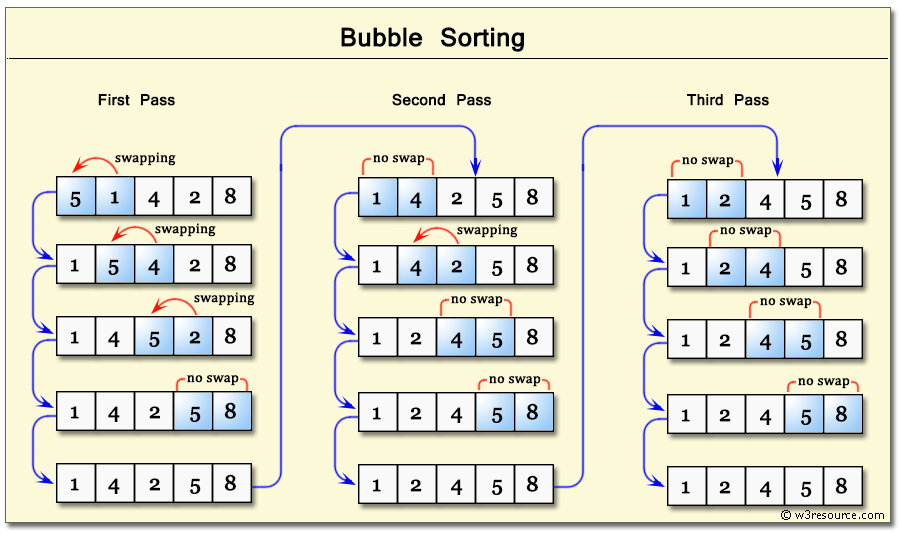
\includegraphics[scale=0.5]{ressources/bubble-sort.png}
        \caption{Exemple graphique d’un tri par bulle}
    \label{fig:fusion}
\end{figure}
\par
Nous pouvons le représenter via le pseudo code suivant :
\par
\begin{function}[H]
    \textbf{Variables :}\\
    i,j : entier\;
    tmp,b : entier\;
    
    
    \Begin{
        \For{$i \leftarrow 1$ \KwTo N-1}{
            $b \leftarrow true$\;
            \While{b} {
            \For{$j \leftarrow i+1$ \KwTo N-1}{
            
            \uIf{tab[j] > tab[j+1]}{
            $b \leftarrow false$\;
                $tmp \leftarrow tab[j]$\;
                 $tab[j] \leftarrow tab[j+1]$\;
                 $tab[j+1] \leftarrow tmp$\;
            }
            }
            }
        }
       
      
    }
    \caption{Bulle(Entrée: tab: tableau d'entier; )}
\end{function}
\section{Calcul de complexité}
\subsection{Complexité temporelle}
Pour le tri a bulle le nombre d'itérations de la boucle externe est compris entre 1 et n. il y a exactement n-1 comparaisons et au pire cas n-1 permutations.

\textbf{Moyenne et Pire Cas:} Le nombre de comparaisons "si Tab[ j-1 ] > Tab[ j ] alors" est une valeur qui ne dépend que de la longueur n de la liste (n est le  nombre d'éléments du tableau), ce nombre est égal au nombre de fois que les itérations s'exécutent, le comptage montre que la boucle "pour i de n jusquà 1 faire" s'exécute n fois (donc une somme de n termes) et qu'à chaque fois la boucle "pour j de 2 jusquà i faire" exécute (i-2)+1 fois la comparaison "si Tab[ j-1 ] > Tab[ j ] alors".

La complexité en nombre de comparaisons est égale à la somme des n termes suivants (i = n, i = n-1,....)

C = (n-2)+1 + ([n-1]-2)+1 +.....+1+0 = (n-1)+(n-2)+...+1 = n(n-1)/2 (c'est la somme des n-1 premiers entiers).

La complexité en nombre de comparaison est de de l'ordre de n², que l'on écrit O(n²).
\par
\textbf{La Meilleur Cas:} (une seule itération) est atteint quand le tableau est déjà trié. Dans ce cas, la complexité est linéaire. O(n)
\subsection{Complexité spatiale}
O(1)
\section{Experimentation}
Le tableau suivant représente les temps d’exécution en nanoseconde de l’algorithme selon la variation de la taille et la configuration de l'entree .
\subsubsection{Les données du tableau sont triées en ordre inverse.}
\small
\begin{center}
\resizebox{19cm}{!}{
\begin{tabular}{| c | c | c | c | c | c | c | c | c | c | c |}
    \hline
    N &  10000 & 50000 & 100000 & 500000 & 1000000 & 5000000 & 10000000 & 50000000 \\
    \hline
    Temp(s) & 0.034025&
0.976482&
4.519502&
115.577318&
//&
//&//&//  \\
    \hline
\end{tabular}}
\end{center}
\normalsize
\subsubsection{Les données du tableau sont triées en bon ordre.}
\small
\begin{center}
\resizebox{19cm}{!}{
\begin{tabular}{| c | c | c | c | c | c | c | c | c | c | c |}
    \hline
    N &  10000 & 50000 & 100000 & 500000 & 1000000 & 5000000 & 10000000 & 50000000 \\
    \hline
    Temp(s) & 0.000009&
0.000034&
0.000084&
0.000274&
0.000704&
0.00361&
//&
//  \\
    \hline
\end{tabular}}
\end{center}
\normalsize
\par
\subsubsection{Les données du tableau sont aleatoires.}
\small
\begin{center}
\resizebox{19cm}{!}{
\begin{tabular}{| c | c | c | c | c | c | c | c | c | c | c |}
    \hline
    N &  10000 & 50000 & 100000 & 500000 & 1000000 & 5000000 & 10000000 & 50000000 \\
    \hline
    Moyenne(s) & 0.09877&
4.081052&
18.926856&
493.184478&
//&
//&
//&
//  \\
    \hline
\end{tabular}}
\end{center}
\normalsize
\par
La figure suivante représente l’évolution du temps d’exécution en (s) selon la taille et la configuration du tableau :
\begin{figure}[H]
    \centering
        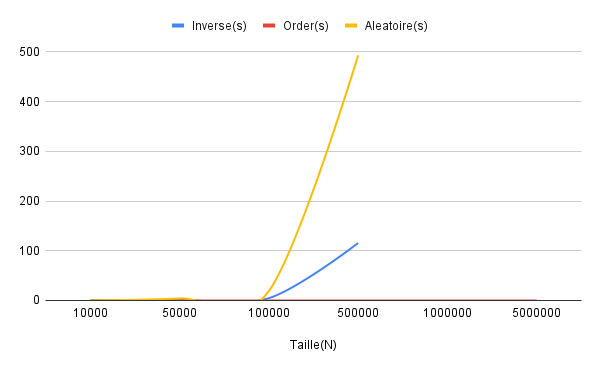
\includegraphics[scale=0.7]{ressources/bulleexp.png}
        \caption{Temps d'exécution du programme selon la taille du tableau}
    \label{fig:temps_exec_dico_theo}
\end{figure} 
\par
Depuis les graphes, on observe que le temps d’exécution évolue de manière quadratique avec l’augmentation de la taille du tableau pour le tri aleatoire et inverse , par contre il s'evolue de maniere linear dans la meilleur cas ( tableau tri en bon ordre) , ce qui correspond bien à la complexité théorique calculée auparavant.
\section{Conclusion}
A partir d'étude expérimentale et théorique de l'algorithme tri a bulle, On constate que malgré sa complexité en temps quadratique sur des données inversées ou triées aléatoirement, il est encore largement utilisé car il est capable de s'exécuter en temps linéaire sur des entrées déjà triées.